\subsection{Theoretical overview of vector boson scattering}\label{ssww13tev:vbs_theory}
VBS processes are very important to understand due to their sensitivity to the EWSB mechanism.
The scattering amplitude of longitudinally polarized vector bosons grows with center-of-mass energy and ultimately violates unitarity above \com{1} in the absence of a light SM Higgs boson~\cite{1977.ben-lee-weak-interactions, 2009.strong-gauge-boson-scattering}.
However, once the Higgs is introduced, the divergences cancel and the cross section no longer grows unbounded, as can be seen in Figure~\ref{fig:ssww13tev_vbs_xsec_higgs}, which consists of plots from~\cite{2008.vbs-resonances-unitarity}.

\begin{figure}[htbp]
  \centering
  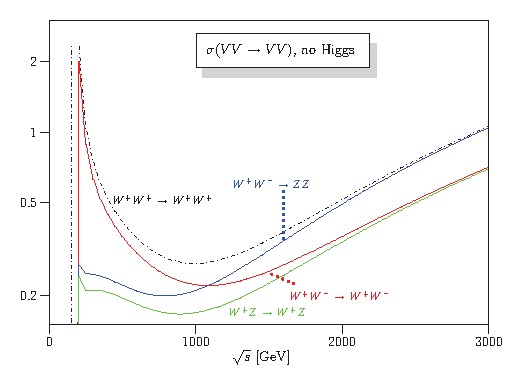
\includegraphics[height=.25\textheight]{figs/ssww_13tev/introduction/vbs_xsec_nohiggs}
  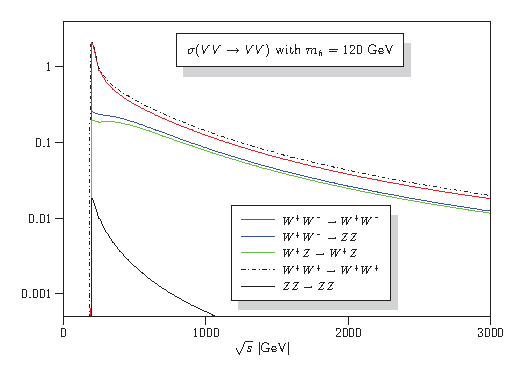
\includegraphics[height=.25\textheight]{figs/ssww_13tev/introduction/vbs_xsec_higgs120}
 
  \caption{Cross sections in nb for five different scattering processes of longitudinally polarized vector bosons.  Without a SM Higgs boson (left), the cross sections grow unbounded with $\sqrt{s}$; however with a $120\gev$ Higgs boson (right), the cross sections no longer diverge.  Plots from~\cite{2008.vbs-resonances-unitarity}. \TODO{properly crop these plots so the rest of the pages aren't visible...}}
  \label{fig:ssww13tev_vbs_xsec_higgs}
\end{figure}

With the discovery of the Higgs boson in 2012~\cite{HIGG-2012-27, CMS-HIG-12-028}, the EWSB mechanism can now be directly studied.
Due to the exchange of a Higgs in the $s$- and $t$-channel VBS diagrams (\ssww specifically only contains the $t$-channel diagram), VBS processes can directly measure properties of the Higgs.
For example, the high-mass tail in the $VV$ scattering system allows an approximation of the effective coupling strength of the Higgs to vector bosons that is independent of any assumptions on the Higgs width~\cite{2015.higgs-constraints-from-vbs}.
Additionally, the center-of-mass energy dependence of the $VV$ scattering can reveal whether the Higgs boson unitarizes the longitudinal scattering amplitude fully or only partially~\cite{2014.higgs-WW-scattering-theory}.

VBS events are characterized by two quarks from the colliding protons each radiating a massive vector boson which then scatter and decay in the detector.
These high-momentum quarks only deflect a small amount upon radiating the vector boson; as a result, they often travel very close to the beam line.
Ignoring the decay products of the bosons, these VBS events result in a final state of two vector bosons ($V$) and two jets ($j$) at high pseudorapidities (called \emph{forward jets}) from the outgoing quarks.
The shorthand $VVjj$ is used to represent this final state.

These $VVjj$ events can be produced via two different physical processes.
The first involves purely electroweak interactions in the tree-level diagrams, with $\mathcal{O}(\alpha_{\textrm{EWK}}) = 6$ %(including the decays of the bosons).
and will be referred to as \emph{EWK production}.
This can be further broken down into VBS and non-VBS production.
In the VBS EWK production, the scattering occurs via triple or quartic gauge couplings, as well as the $s$- or $t$-channel exchange of a Higgs boson.
%These diagrams are shown in Figure~\ref{fig:ssww13tev_diagrams_vbs}.
The non-VBS EWK production contains the same final state of two vector bosons and two outgoing quarks, but the bosons do not scatter.
Due to gauge invariance, it is not possible to separate the VBS from the non-VBS productions~\cite{2006.isolating-vbs-lhc}; therefore, both are included in the signal generation and are indistinguishable from one another.
The second process involves a mix of the EWK and strong interactions, of order $\mathcal{O}(\alpha_s) = 2 \otimes \mathcal{O}(\alpha_{\textrm{EWK}}) = 4$ and will be referred to as \emph{QCD production}.
The tree-level Feynman diagrams for VBS EWK, non-VBS EWK, and QCD $VVjj$ production are found in Figures~\ref{fig:ssww13tev_diagrams_vbs}, \ref{fig:ssww13tev_diagrams_ewk}, and \ref{fig:ssww13tev_diagrams_qcd}, respectively.

\begin{figure}[htbp]
  \centering
  \includegraphics[width=.8\textwidth]{figs/ssww_13tev/diagrams/Vbscore}
  \caption{Tree-level Feynman diagrams for VBS EWK $VVjj$ production including triple gauge couplings involving $W$ and/or $Z$ bosons (top left and top middle), quartic gauge coupling (top right), or the exchange of a Higgs boson ($s$-channel bottom left and $t$-channel bottom right).  The labels are quarks ($q$), fermions ($f$), and gauge bosons ($V = W,Z$). \TODO{Crop properly}}
  \label{fig:ssww13tev_diagrams_vbs}
\end{figure}

\begin{figure}[htbp]
  \centering
  \includegraphics[width=.54\textwidth]{figs/ssww_13tev/diagrams/NoVbsEW}
  \caption{Tree-level Feynman diagrams for non-VBS EWK $VVjj$ production.  The labels are quarks ($q$), fermions ($f$), and gauge bosons ($V = W,Z$). \TODO{Crop properly}}
  \label{fig:ssww13tev_diagrams_ewk}
\end{figure}

\begin{figure}[htbp]
  \centering
    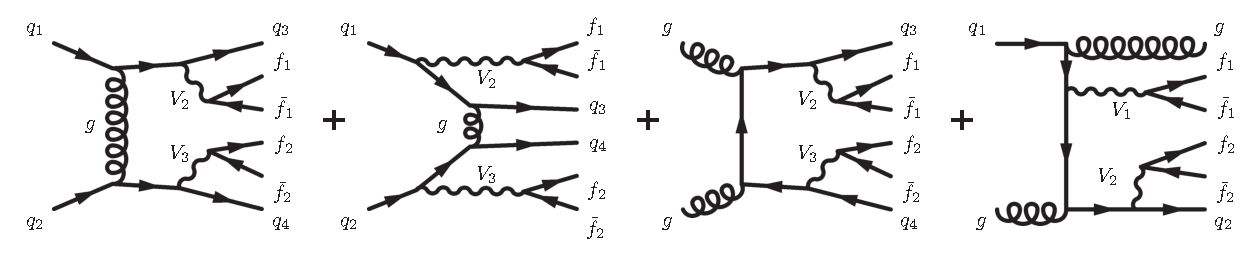
\includegraphics[width=\textwidth]{figs/ssww_13tev/diagrams/VbsQCD}
  \caption{Tree-level Feynman diagrams for QCD $VVjj$ production.  The labels are quarks ($q$), fermions ($f$), and gauge bosons ($V = W,Z$). \TODO{Crop properly}}
  \label{fig:ssww13tev_diagrams_qcd}
\end{figure}

\TODO{Continue here}
Using the \tt{SHERPA} Monte Carlo (MC) generator, leading order cross sections at \com{8} are calculated for a variety of diboson processes
For example, even though the total cross section of opposite-sign $WW$ production is considerably larger than that of same-sign $WW$, the ratio of EWK to QCD production is approximately 3\%
%Therefore, all production modes for \ssww are studied together, with specific selection criteria designed to preferentially select events with a VBS signature.

There are several advantages to studying the same-sign $WW$ process specifically.
The final state's net charge of $\pm 2$ helps considerably in reducing the number of background processes that can mimic the signal.

\begin{table}[htbp]
  \centering
  \begin{tabular}{l r r}
    Process & $\sigma_{\textrm{EWK}}$ & $\sigma_{\textrm{QCD}}$ \\
    \hline\hline
    $W^{\pm}W^{\pm}\rightarrow l^{\pm}l^{\pm}\nu\nu jj$ & 19.5 fb & 18.8 fb \\
    $W^{\pm}W^{\mp}\rightarrow l^{\pm}l^{\mp}\nu\nu jj$ & 91.3 fb & 3030 fb \\
    $W^{\pm}Z\rightarrow l^{\pm}l^{\pm}l^{\mp}\nu jj$   & 30.2 fb & 687 fb  \\
    $ZZ\rightarrow l^{+}l^{-}\nu\nu jj$             & 2.4 fb  & 162 fb  \\
    $ZZ\rightarrow l^{+}l^{-}l^{+}l^{-} jj$           & 1.5 fb  & 106 fb \\
    \hline
  \end{tabular}
  \caption{Predicted cross sections for EQK and QCD production of diboson processes relevant to VBS at \com{8}.  Table from~\cite{2013.ssww-8tev-atlas-support}.}
  \label{tab:ssww13tev_qcd_vs_ewk}
\end{table}

\subsection{Same-sign $W^{\pm}W^{\pm}$ scattering}\label{ssww13tev:ssww_topology}

The process of interest is the production of two $W$ bosons with the same electric charge and two jets.
For the purposes of this analysis, only the case where both bosons decay leptonically to electrons or muons is considered, which results in a final state with two same charge leptons, two neutrinos, and two jets.

% i think i really only need to include the vbs diagrams for ssww (maybe also the ewk?) since the general VV ones are above for all processes
\begin{figure}[htbp]
  \centering
  \includegraphics[width=.32\textwidth]{figs/ssww_13tev/diagrams/vbs1}
  \includegraphics[width=.32\textwidth]{figs/ssww_13tev/diagrams/vbs2}
  \includegraphics[width=.32\textwidth]{figs/ssww_13tev/diagrams/vbs3}
  \caption{Feynman diagrams for VBS EWK production of \ssww events. The leftmost diagram contains a quartic gauge coupling vertex, and the rightmost diagram contains an exchange of a Higgs boson. \TODO{Make own diagrams}}
  \label{fig:ssww13tev_diagrams_vbs_ssww}
\end{figure}

%\begin{figure}[htbp]
%  \centering
%  \includegraphics[width=.32\textwidth]{figs/ssww_13tev/diagrams/ewk1}
%  \includegraphics[width=.32\textwidth]{figs/ssww_13tev/diagrams/ewk2}
%  \caption{Feynman diagrams for non-VBS EWK production of \ssww events. \TODO{Make own diagrams}}
%  \label{fig:ssww13tev_diagrams_ewk}
%\end{figure}

%\begin{figure}[htbp]
%  \centering
%    \includegraphics[width=.32\textwidth]{figs/ssww_13tev/diagrams/qcd1}
%    \includegraphics[width=.32\textwidth]{figs/ssww_13tev/diagrams/qcd2}
%    \includegraphics[width=.32\textwidth]{figs/ssww_13tev/diagrams/qcd3}
%  \caption{Feynman diagrams for QCD production of \ssww events. \TODO{Make own diagrams}}
%  \label{fig:ssww13tev_diagrams_qcd}
%\end{figure}

\begin{figure}[htbp]
  \centering
    \includegraphics[width=.95\textwidth]{figs/ssww_13tev/introduction/vbs_event_topology}
  \caption{\ssww VBS event topology containing two leptons (1 and 2) with the same electric charge, two neutrinos, and two forward tagging jets (3 and 4) with large rapidity separation $\Delta y$.}
  \label{fig:ssww13tev_event_topology}
\end{figure}


%\subsection{}\label{ssww13tev:theory}
%The theoretical motivation for studying the ssWW process is detailed in Section~\ref{ssww13tev:vbs_theory}.
\TODO{Re-write this section referencing the main description in the 13tev section. Maybe just turn this into a 1 or 2 sentence refresher}
The particular interest in polarization is the potential for the scattering amplitude of longitudinally polarized weak bosons to diverge linearly as the center of mass energy increases, ultimately violating unitarity around $1\tev$ \cite{1977.ben-lee-weak-interactions}.
In the Standard Model, the Higgs boson cancels these divergences.
However, as the Higgs is recently discovered it is still extremely to study the mechanism of electroweak symmetry breaking (EWSB), and the longitudinal scattering of $W$ bosons is expected to be one of the most sensitive tests of EWSB~\cite{2013.longitudinal-theory}.

%some additional detail on the interest in the longitudinally polarized $W$ bosons follows \cite{2016.ssww-polarization, 2013.longitudinal-theory, 2017.multiboson-at-lhc}.

\subsection{Experimental sensitivity to longitudinal polarization}\label{sec:sswwupgrade_longitudinal_sens}
\TODO{mention that since there are so many polarization possibilities, a large integrated luminosity is needed to measure just one of them individually}
There are three possible polarization states for a massive vector boson: two transverse ($+$ or $-$) and one longitudinal ($0$).
Therefore, in a system with two $W$ bosons, the overall polarization can be purely longitudinal ($00$), purely transverse ($++$, $--$, and $+-$), or mixed ($+0$ and $-0$).
The three combinations will be referred to as \emph{LL}, \emph{TT}, and \emph{LT} respectively.

In order extract the longitudinal scattering component, it is necessary to find variables that distinguish the LL from the TT and LT.
Several variables were studied, and those with the best discriminating power between the polarizations were the leading and subleading lepton $\pt$ as well as the azimuthal separation ($|\dphijj|$) of the two VBS jets.
The LL events preferred lower $\pt$ for both signal leptons (see Figure~\ref{fig:polarization_leppt}), which motivates keeping these two cuts as low as possible in the event selection in order to preserve as much longitudinal polarization as possible.
In the case of $|\dphijj|$, the LL events generally had a larger dijet separation (see Figure~\ref{fig:polarization_dphijj}), and this variable is used in a binned likelihood fit to extract the longitudinal scattering significance.

\begin{figure}[htp]
  \centering
  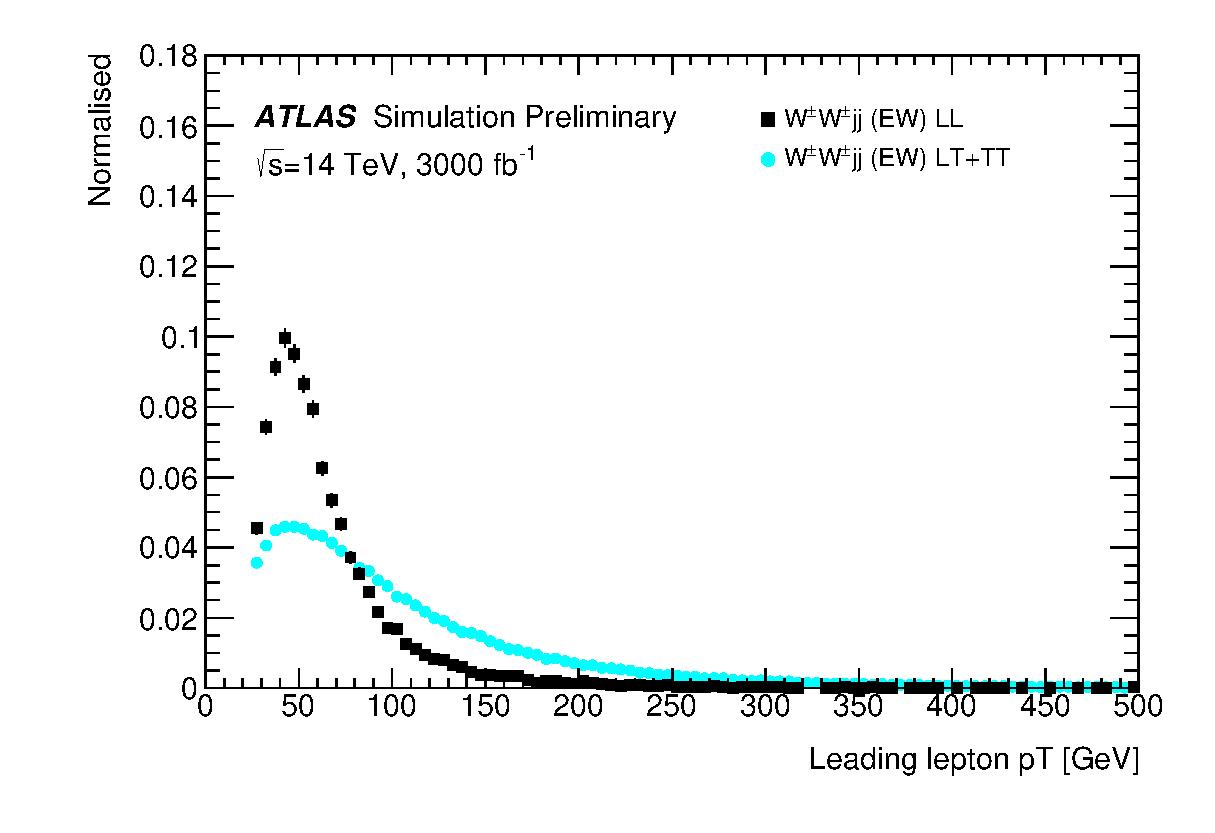
\includegraphics[width=0.8\textwidth]{figs/ssww_upgrade/polarization/lepton0_pt_pass9}\\
  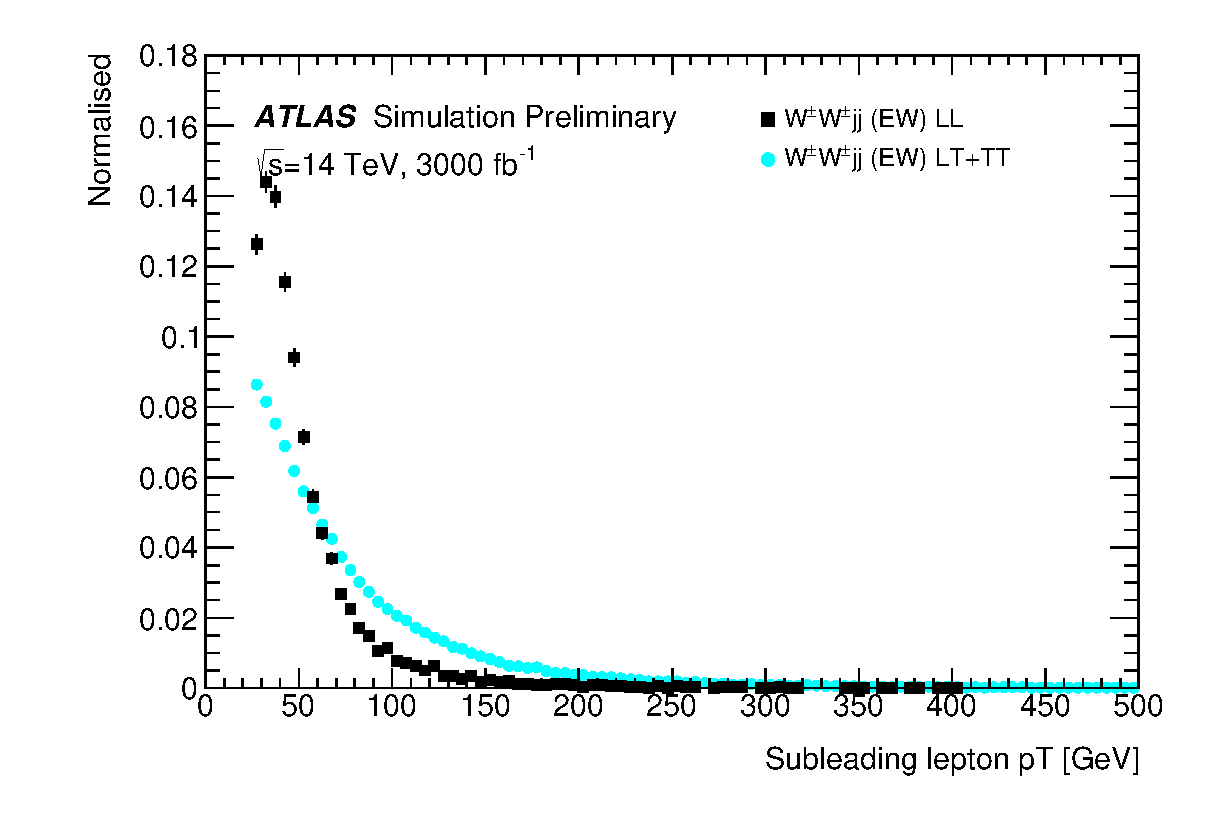
\includegraphics[width=0.8\textwidth]{figs/ssww_upgrade/polarization/lepton1_pt_pass9}
  \caption{Comparison of the leading (top) and subleading (bottom) lepton $\pt$ distributions for purely longitudinal (LL, black) and mixed polarization (LT+TT, cyan) \ssww events.}
  \label{fig:polarization_leppt}
\end{figure}

\begin{figure}[htp]
  \centering
  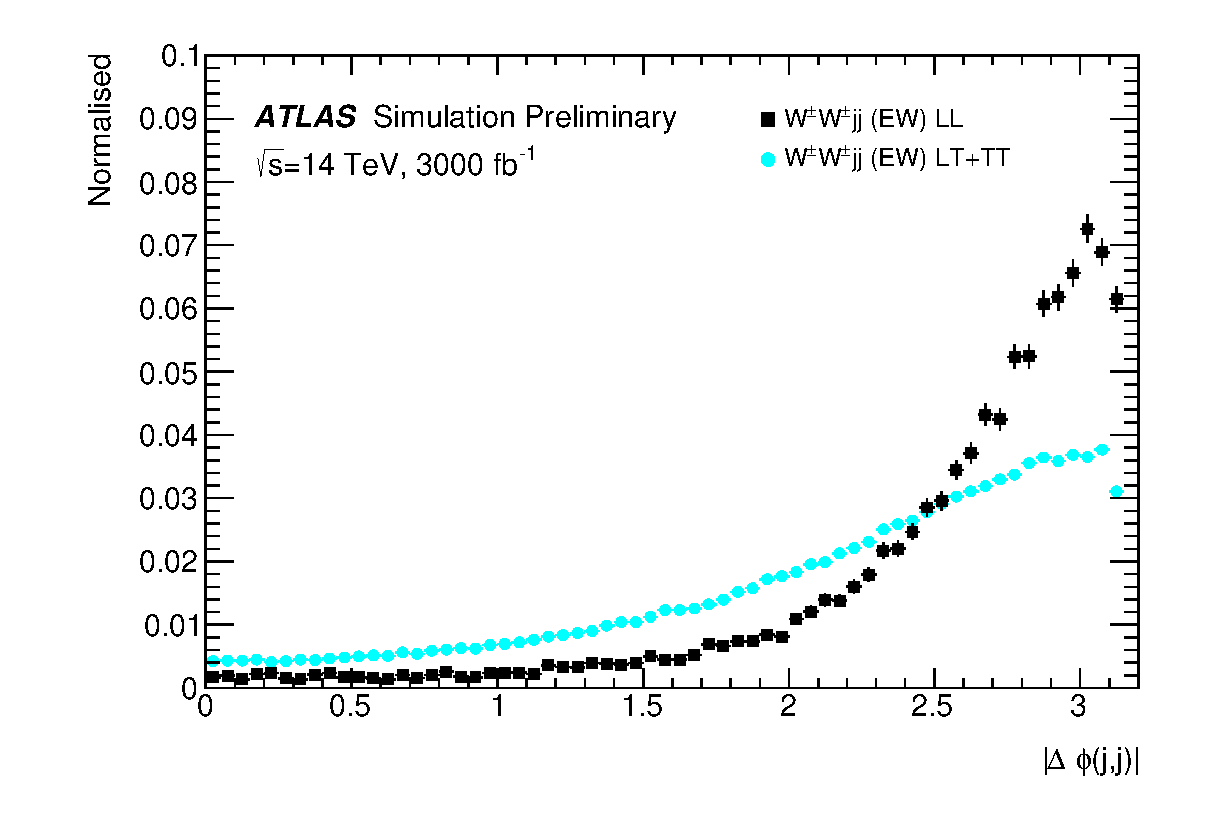
\includegraphics[width=0.8\textwidth]{figs/ssww_upgrade/polarization/dijet_absdphijj_pass9}
  \caption{Comparison of the azimuthal dijet separation ($|\dphijj|$) for purely longitudinal (LL, black) and mixed polarization (LT+TT, cyan) \ssww events.}
  \label{fig:polarization_dphijj}
\end{figure}

